\documentclass[conference,a4paper]{IEEEtran}
% EpiScope technical report (H2). Build: latexmk -pdf main.tex
\IEEEoverridecommandlockouts
\usepackage[T1]{fontenc}
\usepackage{lmodern,microtype,amsmath,amssymb,booktabs,graphicx,xcolor,url,array}
\usepackage[most]{tcolorbox}
\usetikzlibrary{positioning,calc,arrows.meta}
\usepackage[hidelinks]{hyperref}
\setlength{\emergencystretch}{1.5em}
% Draft footer (remove for v1.0)
\usepackage{fancyhdr,lastpage}
\fancyhf{}\renewcommand{\headrulewidth}{0pt}
\fancyfoot[C]{\footnotesize Draft v0.1, 20 Oct 2026 \quad Page \thepage\ of \pageref*{LastPage}}
\pagestyle{fancy}
\newcommand{\repo}{\url{https://github.com/Shinzuu/episcope}}
% Boxes where a member still has to write or confirm. Removed before v1.0.
\newtcolorbox{teammate}[1]{colback=yellow!12,colframe=orange!70!black,boxrule=0.5pt,arc=1pt,
  title={\footnotesize\bfseries TEAMMATE: #1},fonttitle=\footnotesize,left=3pt,right=3pt,top=1pt,bottom=1pt,
  fontupper=\footnotesize}
% Numbers from the provisional test runs (SF=0.05 drill of 11 Oct, SF=0.25 build of 20 Oct); replaced by the v1.0 run.
\newcommand{\prov}{\textsuperscript{\textcolor{orange!70!black}{\scriptsize P}}}

\begin{document}
\title{EpiScope: A Big Data Platform for Disease Surveillance, Forecasting and Response Planning in Bangladesh}
\author{\IEEEauthorblockN{Group [TEAMMATE: number]: Shezan [ID], Tahsin Ahmed Rafi [ID], Rimjhim Dey [ID], Samira [ID]}
\IEEEauthorblockA{CSE 4345 Big Data Analytics, Premier University, Chittagong\\
Repository: \repo\quad Video: [link added at v1.0]}}
\maketitle
\thispagestyle{fancy}

\begin{abstract}
EpiScope turns routine health, climate and logistics data into district-level early warnings, one to four week
forecasts, an allocation of a fixed national stock and a seasonal preparedness calendar. It is built as a Spark
and Delta Lake medallion lakehouse over a synthetic encounter feed of more than 25 million records that takes
its population, geography and weather from real public data. This draft fills the data engineering sections
from the code and the evidence that exists on 20 October 2026; results marked \prov{} come from
provisional test runs (SF=0.05 and SF=0.25) and will be replaced by the tagged v1.0 run.
\end{abstract}

\begin{teammate}{Samira (report lead)}
Draft v0.1. Each yellow box names who writes or confirms that part. Every number must come from a file in
\texttt{docs/experiments/} of the v1.0 run. Page limit: 15 pages plus appendices.
\end{teammate}

\section{Introduction and Problem Analysis}
Bangladesh carries a heavy and strongly seasonal load of infectious disease. The 2023 dengue season was the
worst on record: WHO counted 308,167 cases and 1,598 deaths up to the end of November~\cite{who2023don498}.
Data that could warn earlier already exists, but it sits in separate systems that differ in format,
timeliness and quality, so most analysis happens after hospitals are already full.

The Ministry of Health (a teaching case) asks for a prototype that, for each of the 64 districts, (i) detects
unusual rises in dengue, diarrhoea, influenza-like illness (ILI) and malaria, (ii) forecasts cases and hospital
demand one to four weeks ahead, (iii) allocates a limited national stock, and (iv) gives a preparedness
calendar for the next year. The users are not data scientists, the data is late and incomplete, no patient may
be exposed, and the system must run on a 16\,GB laptop.

\begin{table}[htbp]
\caption{Stakeholders and what the design does for each}
\label{tab:stakeholders}
\centering\footnotesize
\begin{tabular}{@{}>{\raggedright\arraybackslash}p{2.1cm}>{\raggedright\arraybackslash}p{5.6cm}@{}}
\toprule
Stakeholder & Need, and where the design meets it \\
\midrule
MoH policymakers & Defensible allocation: LP against a population baseline, equity floor $\alpha$ \\
Epidemiologists & Transparent methods: EARS C2 and CUSUM, thresholds from a sweep, artefact handling \\
District officers & Early local warning: ranked alert table, district view \\
Hospital managers & Bed and supply demand with 80\% intervals \\
Vector control & Hotspots by district and week; upazila withheld for privacy \\
Patients, public & Keyed hash, age bands, suppression of counts 1 to 4 \\
Privacy regulator & Line-level data never leaves the lake; only aggregates reach the browser \\
\bottomrule
\end{tabular}
\end{table}

\begin{teammate}{Samira}
Risk register (at least 5 risks): start from \texttt{docs/proposal.md} \S6 and update each risk's status. Known
updates: risk 2 (SF=1 within 45 minutes) waits on the scaling run; risk 3 (hidden drop) passed the drill;
risk 7 (uneven commits) has happened.
\end{teammate}

\section{CEP Attributes and Conflict Resolution}
\subsection{Attributes P1 to P7}
\begin{itemize}
\item \textbf{P1 depth of knowledge.} Distributed processing and storage (Spark, Delta, partitioning, broadcast
joins), keyed hashing built from \texttt{sha2}, surveillance statistics (EARS C2, CUSUM), count regression (NB-GLM),
linear programming and visual encoding in D3.
\item \textbf{P2 conflicting requirements.} The five conflicts below, each settled with a number.
\item \textbf{P3 depth of analysis.} Thresholds come from a sweep against injected outbreaks, forecasts from a
52-origin backtest against a baseline, and $\alpha$ from a curve over budgets.
\item \textbf{P4 unfamiliar issues.} Late records (MERGE on the latest report), a facility that goes silent and
back-fills (onset-week counts, missing rather than zero), the same patient at two facilities (DQ-4), and the
Dhaka skew.
\item \textbf{P5 beyond standard codes.} ICD-10 three-character buckets, WHO IDSR~\cite{who2019idsr} for the
diseases and the weekly cadence, and our own suppression and allocation rules where no standard exists.
\item \textbf{P6 stakeholders.} Table~\ref{tab:stakeholders}.
\item \textbf{P7 interdependence.} An error in bronze reaches the dashboard: counting by report date would
create a false outbreak, which would raise forecast demand and move stock. Every gold row carries its bronze
batch IDs, so such an error can be traced back.
\end{itemize}

\subsection{Conflicts C1 to C5}
\textbf{C1 sensitivity against specificity.} We allow at most two false alerts per district-year and take the
most sensitive setting under that limit: EARS C2 at threshold 4.0 finds 97\% of outbreaks with 1.27 false
alerts per district-year\prov{} (Section~\ref{sec:eval}).

\textbf{C2 granularity against privacy.} We publish district by week, not upazila. Every count from 1 to 4 is
hidden, and a second cell is hidden in any row or column with only one hidden cell, so no total reveals it.

\textbf{C3 efficiency against equity.} The LP's equity floor $\alpha$ gives every district a share of each
resource in proportion to its population.
\begin{teammate}{Rafi}
The recommended $\alpha$ and its cost from the curve, once the allocation has real need to allocate.
\end{teammate}

\textbf{C4 freshness against cost.} Forecasts and allocations are weekly decisions, so they run in a daily
batch. Alerts can also run from a Structured Streaming file source that refreshes them as files land
(Section~\ref{sec:data}); between files it holds almost no memory.

\textbf{C5 accuracy against interpretability.} The forecast is a negative-binomial GLM with seasonal terms and
lagged rainfall and temperature: each coefficient can be read as a rate ratio. It beats seasonal naive with a
relative WIS of 0.83\prov.
\begin{teammate}{Rafi}
Confirm whether a more complex model was tried; if not, say so.
\end{teammate}

\section{Architecture and Design Decisions}
EpiScope follows the brief's reference architecture: a medallion lakehouse (bronze, silver, gold) on Apache
Spark~4.0.1~\cite{zaharia2016spark} in local mode with Delta Lake~4.0.1~\cite{armbrust2020delta}, analytics
jobs that read gold and write gold, a serving step that exports suppressed JSON, and a D3.js
v7~\cite{bostock2011d3} dashboard. One command, \texttt{make all}, runs every stage as a small DAG with retries
(\texttt{reference}, \texttt{generate}, \texttt{bronze}, \texttt{silver}, \texttt{gold}, \texttt{analytics},
\texttt{serve}, \texttt{catalog}; Fig.~\ref{fig:arch}); Java~17 and Python~3.12 come from \texttt{mise.toml} and every Python package
is pinned in \texttt{requirements.txt}. Table~\ref{tab:alternatives} lists the main alternatives and why each was rejected.

\begin{figure}[htbp]
\centering
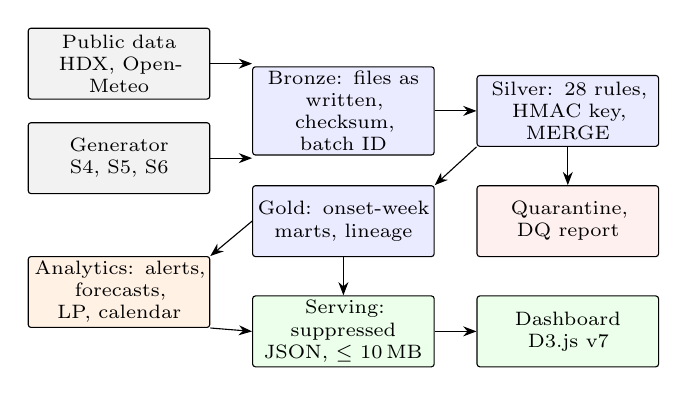
\begin{tikzpicture}[font=\scriptsize, >=Stealth,
  box/.style={draw, rounded corners=1pt, align=center, text width=22mm, minimum height=9mm, inner sep=1.5pt, fill=#1},
  box/.default=white]
\node[box=gray!10]  (pub) at (0,0)     {Public data\\HDX, Open-Meteo};
\node[box=gray!10]  (gen) at (0,-1.2)  {Generator\\S4, S5, S6};
\node[box=blue!8]   (br)  at (2.85,-0.6) {Bronze: files as\\written, checksum,\\batch ID};
\node[box=blue!8]   (si)  at (5.7,-0.6)  {Silver: 28 rules,\\HMAC key, MERGE};
\node[box=red!6]    (qu)  at (5.7,-2.0)  {Quarantine,\\DQ report};
\node[box=blue!8]   (go)  at (2.85,-2.0) {Gold: onset-week\\marts, lineage};
\node[box=orange!10](an)  at (0,-2.9)  {Analytics: alerts,\\forecasts, LP, calendar};
\node[box=green!8]  (se)  at (2.85,-3.4) {Serving: suppressed\\JSON, $\le$ 10\,MB};
\node[box=green!8]  (da)  at (5.7,-3.4)  {Dashboard\\D3.js v7};
\draw[->] (pub.east) -- (br.west |- pub.east);
\draw[->] (gen.east) -- (br.west |- gen.east);
\draw[->] (br) -- (si);
\draw[->] (si) -- (qu);
\draw[->] (si.south west) -- (go.north east);
\draw[->] (go.west) -- (an.north east);
\draw[->] (an.south east) -- (se.west);
\draw[->] (go) -- (se);
\draw[->] (se) -- (da);
\end{tikzpicture}
\caption{EpiScope data flow. Blue: Delta lakehouse on Spark; one Makefile runs every stage.}
\label{fig:arch}
\end{figure}


\textbf{Delta rather than plain Parquet.} Late records (up to 21 days) must update their epi-week without
duplicates. Delta's ACID MERGE makes that a single atomic statement, \texttt{replaceWhere} rewrites only the
changed weeks of gold, and the transaction log gives time travel for ``what did we know on date $t$''.
Iceberg would also work; Delta has the documented pairing with Spark~4.0.1 and pip packaging.

\textbf{Local filesystem rather than HDFS or an object store (ING-5 not done).} A Docker HDFS or S3 store costs
1--2\,GB of RAM that Spark needs on the target laptop. All paths come from two environment variables, so the
lake can move to another URI without code changes.

\textbf{Partitioning.} Bronze is partitioned by \texttt{batch\_id}, because silver reads exactly one new batch
at a time. Silver encounters and gold \texttt{cases\_weekly} are partitioned by \texttt{epi\_year} only: one year
of gold holds at most $64\times4\times53$ rows, so a finer key (district or week) would create thousands of
tiny files at SF=1 without saving any reads. The proposal planned \texttt{division} as a second key; we
dropped it for the same reason.

\textbf{Catalog.} The jobs read and write by path, and a separate \texttt{make catalog} step registers every
table as an external table (\texttt{bronze.encounters}, \texttt{gold.cases\_weekly}, \dots) in a Hive
metastore stored inside the lake. Derby allows one process at a time, so keeping the catalog out of the jobs
means a locked metastore can never stop the pipeline.

\textbf{Orchestration (ENG-4).} \texttt{scripts/dag.py} runs the stages in dependency order and retries a
failed stage twice, 30\,s and then 60\,s later, before it stops; each run leaves a JSON record of attempts and
times in the lake. Retrying is safe because every stage is idempotent: bronze skips files it has already
loaded, silver merges and gold rebuilds only changed weeks. The 170 unit tests (\texttt{make test}, gate 1 of \texttt{make check}) cover the generator, the quality
rules, de-identification and suppression, idempotent loads, detection, forecasting, the LP constraints, the
SEIR fit, the dashboard export and the DAG.

\begin{table}[htbp]
\caption{Alternatives considered}
\label{tab:alternatives}
\centering\footnotesize
\begin{tabular}{@{}>{\raggedright\arraybackslash}p{1.5cm}>{\raggedright\arraybackslash}p{1.5cm}>{\raggedright\arraybackslash}p{4.4cm}@{}}
\toprule
Chosen & Rejected & Reason \\
\midrule
Python DAG behind \texttt{make} & Airflow, Prefect & Airflow needs 4--8\,GB of RAM; Prefect is a new dependency for eight stages \\
Delta Lake & Iceberg, plain Parquet & MERGE and time travel with documented Spark~4.0.1 support; Parquet has neither \\
Batch, plus a streaming refresh & Streaming only & Decisions are weekly; the stream (Section~\ref{sec:stream}) reuses the batch code for alerts \\
Local filesystem & HDFS, MinIO & 1--2\,GB of RAM saved on a 16\,GB laptop \\
Static JSON & An API server & Under 10\,MB of aggregates; nothing to run or secure \\
\bottomrule
\end{tabular}
\end{table}

\section{Data Generation, Quality, Lineage and Privacy}\label{sec:data}

\subsection{Public sources and the generator}
District boundaries, codes and the 2022 census population by age band and sex come from the HDX COD-AB and
COD-PS datasets~\cite{hdx2025codab}; daily precipitation, temperature and humidity at each district centroid
for 2021--2025 come from the Open-Meteo archive~\cite{zippenfeld2023openmeteo}. Open-Meteo allows about 5,000
weighted calls an hour and 64 districts over five years cost about 8,400, so the download is throttled and the
processed reference files (0.6\,MB) are committed. A clean clone therefore skips a two-hour download.

The generator (\texttt{generator/}) writes the three synthetic sources: encounters (S4) as one CSV folder per
report date, a register of 736 facilities (S5) and daily stock snapshots (S6) as JSON. It is vectorised numpy,
seeded per (seed, stream, district, year), so the same arguments give byte-identical output whatever the number
of worker processes. Rates are per head of population, so the row count follows the census rather than a
constant: SF=1 gives about 6.2 million encounters a year, or about 31 million for 2021--2025.

Each disease has its own annual cycle. Dengue peaks in early October, because OpenDengue's national counts peak
in October in 2022 and 2024, later than ``follows the monsoon'' suggests. Dengue responds to rainfall and
temperature four to eight weeks earlier, diarrhoea spikes after extreme rainfall, malaria is concentrated in
the three Hill Tracts districts and Cox's Bazar, and every count has negative-binomial noise. Reporting delay is
a discretised negative binomial with mean 3 days truncated at 21, and 65\% of Friday and Saturday reports move
to Sunday (Bangladesh's weekend). The SF=0.05 run injected 35 outbreaks\prov{} of different shape and size,
including a slow-growing one and a nationwide novel respiratory surge, and two reporting artefacts: a facility
that goes silent for three weeks and then back-fills. They are written only to \texttt{ground\_truth/}, which
the detection code never reads (a test fails if it does).

The generator also plants the defects the quality rules must catch: 2\% repeated \texttt{encounter\_id},
0.5\% orphan \texttt{facility\_id}, 0.5\% invalid age, 0.5\% invalid sex, 0.3\% malformed ICD-10 codes and
0.3\% onsets after the report date. A 14-day incremental drop (\texttt{make drop}) uses the same layout and
carries records with onsets up to 21 days before the drop.

\subsection{Bronze: keep what arrived}
\texttt{pipeline/bronze/ingest.py} finds files by glob, never by name, date or count. It computes each file's
SHA-256 and skips any file whose checksum is already in the ingest log, so a re-run reads nothing and a new
drop loads only its own files. Every value of the contract fields is kept as a string, exactly as written, and
each row gets the source, its file, the checksum, the batch ID and the load time (ING-1). One run is one batch;
batch IDs start with a UTC timestamp, so they sort in load order.

\subsection{Silver: rules, quarantine and de-identification}
The rule catalogue (\texttt{pipeline/quality/rules.py}) has 14 rules for encounters and 7 each for facilities
and stock (DQ-1). Each rule is a Spark column expression that is true when a row breaks it, with a stable reason
code, a severity (quarantine or warn) and the requirement it serves. The six planted defects map one to one onto
six rules:
\begin{itemize}
\item \texttt{DQ\_DUP\_ENCOUNTER} and \texttt{DQ\_ORPHAN\_FACILITY};
\item \texttt{DQ\_INVALID\_AGE} and \texttt{DQ\_INVALID\_SEX};
\item \texttt{DQ\_ONSET\_AFTER\_REPORT} and \texttt{DQ\_BAD\_ICD10}.
\end{itemize}
The rest cover nulls, types, long delays, future dates and outcome values. Spark~4 runs in ANSI mode, where a plain cast of a bad
string throws, so every rule reads values through \texttt{try\_cast} and an unparseable value is a defect of
its own. A failing row goes to \texttt{silver.quarantine} once, with the list of every code it broke. In the
first SF=0.05 load, 66,979 of 1,681,896 encounter rows (4.0\%)\prov{} were quarantined. Each load writes one
row of rule pass rates to \texttt{gold.dq\_report}, which the dashboard shows (DQ-2).

Before a clean row is stored, \texttt{patient\_id} becomes an HMAC-SHA256 under a key held only in
\texttt{.env} (PRV-1). Spark has no HMAC function and a Python UDF over 25 million rows is slow, so the HMAC is
built from Spark's native \texttt{sha2} with the RFC~2104 inner and outer pads. A plain salted hash would not be
enough: national IDs are few enough to enumerate, so the secret key is the only protection. The code refuses to
run with a missing key or the placeholder from \texttt{.env.example}. Exact age becomes an age band.

\subsection{Idempotent incremental loads (ING-4)}
Clean rows are merged into \texttt{silver.encounters} with a Delta MERGE on \texttt{encounter\_id}. A matched
row is replaced only when the incoming \texttt{report\_date} is later. That one condition gives both required
properties: re-running a batch matches every row with an equal date and changes nothing, and a resubmitted or
late record replaces the old copy and moves to its own onset week. The MERGE is limited to the epi-years in the
batch (plus one either side), so partition pruning keeps it from scanning the whole table.

Silver records the weeks each batch changed: the onset weeks of new and replaced rows and the old weeks of
replaced rows. Gold rebuilds only those weeks, plus the week after each, with a Delta \texttt{replaceWhere}.

\subsection{Gold, lineage and patient de-duplication}
\texttt{gold.cases\_weekly} counts cases, admissions, deaths and lab confirmations per district, disease and
ISO week of \emph{onset}. Counting by onset rather than report date is what keeps the back-filled weeks of the
silent facility from looking like an outbreak. Every district-week with at least one reporting facility gets a
row for all four diseases, so a missing row means ``nothing reported'' rather than zero, which the detector
uses to treat silent weeks as missing (AN-3). Each row carries the sorted bronze batch IDs of the records it
counts, which link through the ingest log to file names and checksums (DQ-3).

Cross-facility patient de-duplication (DQ-4) flags a record as a repeat when the same patient key, disease,
sex and compatible age band appear at another facility within seven days. On SF=0.05 it flagged 441 pairs, of
which 440 were true repeats (precision 0.998)\prov{}. Recall within the window was only 0.11\prov{}, because the
generator draws age and sex afresh for a repeat visit, so most planted repeats fail the attribute check. We
kept the strict rule: a false merge would hide a real case.

\subsection{Hidden-drop drill}
\texttt{scripts/hidden\_drop\_drill.sh} rehearses the instructor's test: clone, \texttt{make setup},
\texttt{make all}, a new 14-day drop with an unseen seed, the incremental steps, then the same steps again. On
11 October at SF=0.05 it passed every check\prov{}: the drop was one new bronze batch, silver gained 8,292 rows,
the data moved from 31 December 2025 to 14 January 2026, the re-run changed nothing and left zero duplicate IDs
and zero duplicate gold keys, and the export was 9.64\,MB with no count from 1 to 4. It took 22 minutes,
including setup.

\section{Analytics Methods}
The code below exists and is tested; the leads write the method justification.

\textbf{Detection (AN-1, AN-3).} EARS C2~\cite{hutwagner2003ears} runs on seasonally adjusted, completeness-scaled
weekly counts with Spark window functions; CUSUM runs per district and disease in \texttt{applyInPandas}.
Farrington~\cite{farrington1996} was ruled out because it needs about five years of history before its first
test week. Silent facility-weeks are treated as missing, not zero.

\textbf{Forecasting (AN-4).} One negative-binomial GLM per district for dengue and diarrhoea, with weather
lagged at least as far as the horizon, fitted in parallel through a cogrouped \texttt{applyInPandas}.

\textbf{Demand, allocation and calendar (AN-6, AN-7, AN-9).} Forecast quantiles become beds, IV saline, NS1 kits,
ORS and antimalarials with the assumptions in \texttt{analytics/forecast/demand\_assumptions.py}; the brief's LP
is solved with PuLP~3.3.2 and CBC; STL per division and disease gives the onset and peak weeks.

\begin{teammate}{Rafi}
Write the justification of each method from the literature, the LP formulation with our normalisation per
resource, and what $\alpha$ means for policy. Check the allocation first: in the SF=0.05 run the national net
need was 0 for beds, IV saline, NS1 kits and ORS, so the LP had almost nothing to allocate.
\end{teammate}

\section{Evaluation}\label{sec:eval}
The detection and backtest numbers come from the SF=0.25 build with real weather (seed 42) of 20
October\prov{}, in the detection trade-off and backtest metric files under \texttt{docs/experiments}.

\subsection{Detection}
\texttt{make evaluate} scores every alert against the 35 injected outbreaks in \texttt{ground\_truth/}, the only
code allowed to read that folder. Consecutive alert weeks merge into one episode; an episode that overlaps no
outbreak window counts as a false alert. The sweep picks, for each method, the most sensitive setting that keeps
false alerts at or below two per district-year. Table~\ref{tab:detection} shows the chosen operating points.

\begin{table}[htbp]
\caption{Detection at the chosen operating points (SF=0.25)\prov}
\label{tab:detection}
\centering\small
\begin{tabular}{@{}lrr@{}}
\toprule
 & EARS C2 & CUSUM \\
\midrule
Setting & threshold 4.0 & $k=0.5$, $h=6$ \\
Outbreaks detected & 34 of 35 & 32 of 35 \\
Sensitivity & 0.97 & 0.91 \\
False alerts per district-year & 1.27 & 1.49 \\
Positive predictive value & 0.22 & 0.28 \\
Median days to detection & 8 & 9 \\
Detected within 14 days & 0.91 & 0.83 \\
\bottomrule
\end{tabular}
\end{table}

EARS C2 is the better default here: it finds more outbreaks, sooner, with fewer false alerts. We expected CUSUM
to do better on slow growth, but on the one slow outbreak both methods found it late, EARS C2 after 48 days and
CUSUM after 69.

\begin{teammate}{Samira (AN-2), Rafi (AN-3): confirm}
Add the C1 trade-off figure from \texttt{detection\_tradeoff.csv} (sensitivity against false alerts per
district-year, one curve per method, the chosen points marked), results by outbreak shape, and the artefact
facility with the naive detector and with ours. Replace with the v1.0 numbers.
\end{teammate}

\subsection{Forecast backtest}
The backtest refits the per-district NB-GLM at 52 rolling origins (every fourth origin, reused in between) and
forecasts one to four weeks ahead using only data up to each origin. The seasonal-naive baseline is scored on
exactly the same district, disease, origin and horizon cells. The weighted interval score~\cite{bracher2021wis}
uses eleven central intervals plus the median; relative WIS below 1 means the model beats the baseline.

\begin{table}[htbp]
\caption{Backtest over 52 origins, model against seasonal naive (SF=0.25)\prov}
\label{tab:backtest}
\centering\small
\setlength{\tabcolsep}{4pt}
\begin{tabular}{@{}llrrrr@{}}
\toprule
Disease & $h$ & MAE & MAE base & Cov.\,80\% & Rel.\ WIS \\
\midrule
Dengue & 1 & 39.4 & 42.5 & 0.83 & 0.88 \\
 & 4 & 41.4 & 44.9 & 0.82 & 0.89 \\
Diarrhoea & 1 & 18.5 & 26.3 & 0.80 & 0.70 \\
 & 4 & 19.3 & 26.4 & 0.80 & 0.74 \\
\midrule
All & 1--4 & 29.5 & 35.0 & 0.81 & 0.83 \\
\bottomrule
\end{tabular}
\end{table}

The model beats the baseline at every horizon for both diseases, by more for diarrhoea (relative WIS 0.72)
than for dengue (0.88). Its 80\% intervals cover 81\% of outcomes overall, against 78\% for the baseline, so
the bands mean what they say.

\begin{teammate}{Samira (AN-5): confirm}
Horizons 2 and 3 are in \texttt{backtest\_metrics.csv}. Add the WIS decomposition (for dengue, most of the model's WIS
is underprediction, which matters for stock planning). Replace with the v1.0 numbers.
\end{teammate}

\subsection{Allocation against the population baseline}
\begin{teammate}{Rafi}
In the SF=0.25 run the national net need is zero for beds, IV saline, NS1 kits and ORS, and 8.8 courses of
antimalarials, because the generated stock exceeds the forecast demand. The LP's ``50\% of need met against 1\%
for the population baseline'' is therefore about antimalarials only. Fix the demand or stock assumptions, then
report share of need met and the worst-covered district at five budgets, and the efficiency and equity curve.
\end{teammate}

\subsection{Scalability and Spark optimisations}
\texttt{scripts/scaling.sh} builds each scale factor from a fresh clone and times every stage
(Table~\ref{tab:scaling}). The laptop has an Intel Core i5-8350U (4 cores, 8 threads) and 15.4\,GB of RAM;
Spark runs as \texttt{local[4]} with a 5\,GB driver. SF=1 finishes in 28.3 minutes, inside the 45-minute
gate. Silver grows with the row count and is the slowest stage at SF=1; analytics stays near 7 to 8 minutes at
every scale, because it works on weekly series per district, not on rows. A first SF=1 attempt failed in silver
when Spark's spill filled the small RAM-backed \texttt{/tmp}; spill now goes to a disk folder.

\begin{table}[htbp]
\caption{Minutes per stage from a fresh clone}
\label{tab:scaling}
\centering\small
\setlength{\tabcolsep}{4pt}
\begin{tabular}{@{}lrrr@{}}
\toprule
 & SF=0.25 & SF=0.5 & SF=1 \\
\midrule
Encounter rows (M) & 8.5 & 17.1 & 34.1 \\
Generate & 0.2 & 0.4 & 0.6 \\
Bronze & 1.9 & 2.8 & 4.3 \\
Silver & 3.8 & 6.7 & 11.1 \\
Gold & 1.8 & 2.3 & 3.5 \\
Analytics & 6.9 & 7.1 & 8.0 \\
Serve & 0.7 & 1.1 & 0.9 \\
\midrule
Total & 15.4 & 20.4 & 28.3 \\
Raw / silver (GB) & 1.2 / 0.8 & 2.2 / 1.5 & 4.1 / 2.9 \\
\bottomrule
\end{tabular}
\end{table}

One optimisation is measured. The silver job evaluated the 14 encounter quality rules, including the
duplicate-ID rule that sorts the whole load, once for every output (quarantine, its count, the quality report
and the clean MERGE). It now evaluates them once and persists the result. At SF=0.25 silver's Spark time fell
from 325\,s to 214\,s, and every silver table kept the same row count and row hash
(\texttt{silver\_optimisation.json}).

\begin{teammate}{Samira (ENG-3)}
Spark UI screenshots from the SF=1 event log (kept outside the repository; it holds the padded HMAC key), the
bottleneck stage, and a second optimisation with before and after numbers (candidates: AQE skew handling or
salting on the Dhaka load; backtest parallelism, 365\,s at SF=1 on 4 of 8 threads).
\end{teammate}

\section{Dashboard Design and Usability}
The dashboard (\texttt{dashboard/}) uses only D3.js v7 and the TopoJSON client, both vendored with
subresource-integrity hashes. It loads only the aggregated JSON exports, which must stay under 10\,MB: the
export keeps the most recent weeks that fit. Five views are linked: a district choropleth of incidence per
100,000 with alert markers, a weekly time series with a brush, forecast and bands, a seasonal heatmap, an
allocation view with a what-if panel, and a ranked early-warning table. Suppressed cells are hatched and every
view shows the data-freshness time.
\textbf{Design rationale.} Incidence uses the viridis scale, which stays ordered in greyscale and for the
common colour-vision deficiencies; alerts use the Okabe--Ito vermillion, which stands out against it. Counts
are shown per 100,000 on the map, so a large district does not look worse only for being large, but as raw
cases on the time series, which is what a store-keeper plans with. Suppressed cells are hatched rather than
left blank, so ``hidden'' never reads as ``zero''. Every forecast carries its 80\% band. District by week is
the finest level shown: it is what an officer acts on and the coarsest level that still locates an outbreak.
Below 560\,px the views stack in one column for a phone.

\textbf{District view (PRV-3).} Opening the dashboard with \texttt{?district=} and a district code loads that
district's bundle: its own series, alerts, forecast and allocation in full, and the rest of the country drawn
lighter as division totals.

% PERSONA: simulated persona walkthroughs (step 4)

\section{Ethical, Societal and Sustainability Considerations}
\textbf{Privacy by design.} No real patient data is used; every encounter is synthetic and labelled so.
Direct identifiers stop at bronze: silver and gold hold only the keyed hash and age bands, the key never enters
Git, and every export hides counts from 1 to 4 with complementary suppression, so a total cannot reveal a hidden
cell. One residual risk is known and written in the code: the padded HMAC key appears in Spark's query plan, so
Spark event logs of the silver job must be treated as secret and kept outside the repository.

\textbf{Record-level extracts and public release (PRV-4).} \texttt{pipeline/privacy/kanon.py} measures
k-anonymity~\cite{sweeney2002k} over the quasi-identifiers (age band, sex, district, onset week, disease,
facility) of any record-level extract. k-anonymity does not stop a homogeneity attack, where everyone in a class
shares one diagnosis, so a disease extract also needs l-diversity. For a public release, differential
privacy~\cite{dwork2006dp} is the stronger tool: the Laplace mechanism adds noise with standard deviation
$\sqrt{2}/\varepsilon$ to each count, about 1.4 cases at $\varepsilon=1$. The privacy budget adds up over every
published cell and week, and noisy counts can be negative and must be post-processed. We would use it for the
public release only; ministry users keep exact counts with suppression.
\begin{teammate}{Samira: confirm}
Equity (what $\alpha$ protects and what it costs), misuse (stigma of a named district, alert fatigue), the
limits of big-data signals~\cite{lazer2014flu}, and the energy and hardware footprint.
\end{teammate}

\section{Limitations and Future Work}
The data is synthetic, so detection and forecast scores measure how well the methods recover patterns we
planted, not real-world accuracy. The storage layer runs on the local filesystem, not HDFS or an object store
(ING-5). Patient de-duplication is precise but misses most repeats whose age or sex was recorded differently.
\begin{teammate}{All}
Add each area's main limitation and one concrete next step.
\end{teammate}


\bibliographystyle{IEEEtran}
\bibliography{refs}

\appendices
\section{Policy Brief for the Director}
\begin{teammate}{Samira, two pages, no jargon}
Current situation; top three recommendations with expected impact; how to read the dashboard; confidence and
limitations; data-protection assurance.
\end{teammate}

\section{Contribution Matrix}
\begin{teammate}{All, agreed and signed}
Work areas from Appendix B of the brief, one column per member (L, S or none), agreed share $\sigma_i$ (total
100), commits and lines from \texttt{git shortlog -sn}, signatures. Ask the instructor to confirm that the
moderation factor uses $N=4$.
\end{teammate}

\section{Individual Reflections}
\begin{teammate}{Each member writes their own half page}
Shezan, Rafi, Rimjhim, Samira.
\end{teammate}

\end{document}
